% ============================================================================
% SEC03.TEX - Section 2.3: Unity Editor Interface
% ============================================================================

\section{Unity Editor Interface}

\begin{learningoutcomes}
\item Mengenal semua panel utama Unity Editor
\item Memahami fungsi setiap panel
\item Mampu mengatur layout editor
\item Mampu melakukan navigasi dasar di Unity Editor
\end{learningoutcomes}

\subsection{Panel Utama Unity Editor}

\begin{figure}[ht]
    \centering
    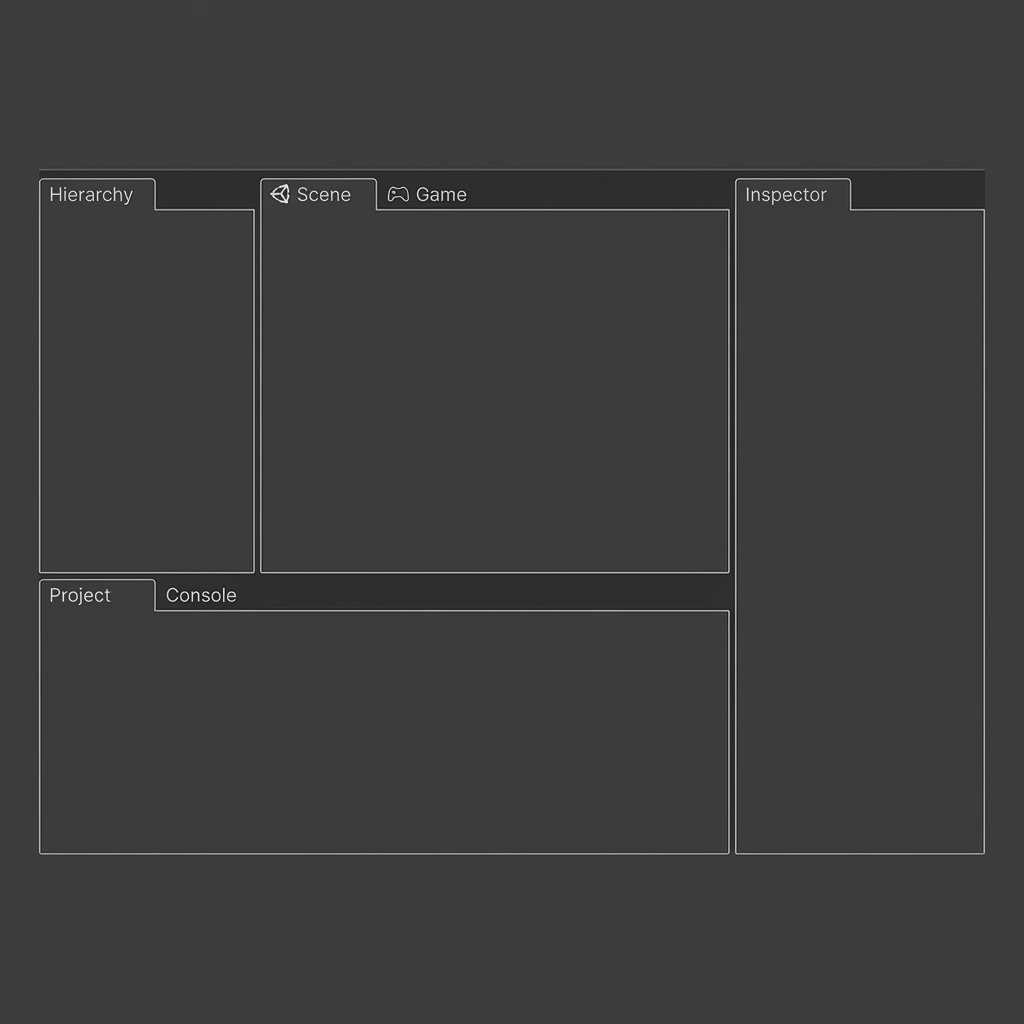
\includegraphics[width=\textwidth]{figures/unity_editor.png}
    \caption{Layout Standar Unity Editor}
    \label{fig:unity_editor}
\end{figure}

\subsubsection{1. Scene View}
Area untuk mengedit dan mengatur scene:
\begin{itemize}
\item Navigasi: Pan (Q), Rotate (E), Scale (R), Move (W)
\item Gizmos untuk manipulasi objek
\item View tools untuk navigation
\end{itemize}

\subsubsection{2. Game View}
Preview bagaimana game akan terlihat saat dimainkan:
\begin{itemize}
\item Aspect ratio testing
\item Resolution testing
\item Play mode preview
\end{itemize}

\subsubsection{3. Hierarchy}
Menampilkan semua GameObject dalam scene aktif:
\begin{itemize}
\item Struktur parent-child
\item Drag-and-drop untuk mengatur hierarchy
\item Search dan filter
\end{itemize}

\subsubsection{4. Inspector}
Menampilkan properti GameObject atau asset yang dipilih:
\begin{itemize}
\item Component properties
\item Transform values
\item Script variables
\end{itemize}

\subsubsection{5. Project}
File browser untuk semua assets dalam project:
\begin{itemize}
\item Folder structure
\item Asset preview
\item Search dan filter
\end{itemize}

\subsubsection{6. Console}
Menampilkan log, warning, dan error:
\begin{itemize}
\item Debug messages
\item Error tracking
\item Clear logs
\end{itemize}

\subsection{Layout Customization}

Unity memungkinkan customisasi layout:
\begin{itemize}
\item Window $\rightarrow$ Layouts untuk preset layouts
\item Drag panel untuk mengatur posisi
\item Save custom layout
\end{itemize}

\subsection{Shortcuts Penting}

\begin{itemize}
\item \textbf{Ctrl/Cmd + S}: Save scene
\item \textbf{Ctrl/Cmd + Shift + N}: New GameObject
\item \textbf{F}: Focus pada objek terpilih
\item \textbf{Space}: Play/Pause
\item \textbf{Ctrl/Cmd + Shift + C}: Clear Console
\end{itemize}

\begin{catatan}
Menguasai shortcuts akan mempercepat workflow. Gunakan Edit $\rightarrow$ Shortcuts untuk melihat dan mengubah shortcuts.
\end{catatan}
